\chapter{Конструкторская часть}
В данном разделе формализуются требования к программному обеспечению, объекты сцены и их структура, приводится декомпозиция задачи, а также рассматриваются схемы алгоритмов визуализации сцен объектов методом трассировки лучей.

\section{Требования к программному обеспечению}
Пользовательский интерфейс разрабатываемой программы должен предоставлять следующие функциональные возможности:
\begin{itemize}
	\item возможность выбора визуализируемой сцены из трех предложенных вариантов: сцена с двумя сферами, сцена с кубом, сферой и фигурой коня, сцена со всеми шахматными фигурами;
	\item возможность выбора объекта сцены путем нажатия на него мышкой или его выбора в списке объектов;
	\item возможность изменения цвета и коэффициента отражения выбранного объекта сцены;
	\item возможность выбора типа закраски объекта: по методу Гуро и по методу Фонга;
	\item возможность включения режима глубины поля, при этом возможно изменение расстояния от камеры до фокальной точки;
	\item возможность включения режима сглаживания изображения.
\end{itemize}

К разработанному ПО предъявляются следующие требования:
\begin{itemize}
	\item чтение моделей шахматных фигур производится из объектных файлов при первом построении выбранной сцены в рамках одного запуска программы, модели шахматных фигур представлены полигональной сеткой;
	\item модели шара и куба представляются в программе аналитически;
	\item программа должна корректно обрабатывать ввод некорректных данных.
\end{itemize}

\section{Формализация объектов синтезируемой сцены}
Синтезируемые сцены состоят из следующих типов объектов:
\begin{itemize}
	\item точечный источник света, представимый положением в пространстве и интенсивностью;
	\item сфера, представимая точкой центра и радиусом;
	\item куб, грани которого параллельны координатным плоскостям. В программе представлен точкой центра и длиной стороны;
	\item шахматные фигуры: король, ферзь, ладья, слон, конь и пешка. Фигуры описываются точкой положения центра нижней грани, а также массивом треугольных полигонов, из которых составлена фигура. Треугольные полигоны, в свою очередь, описаны тремя вершинами и тремя нормалями в этих вершинах;
	\item камера, характеризуемая положением в пространстве и направлением вектора наблюдения.
\end{itemize}


\section{Декомпозиция задачи}
В результате декомпозиции задачи были получены подзадачи, показанные на рисунке~\ref{fig:IDEF0_top}~-~\ref{fig:IDEF0_2}.

\begin{figure}[H]
	\centering
	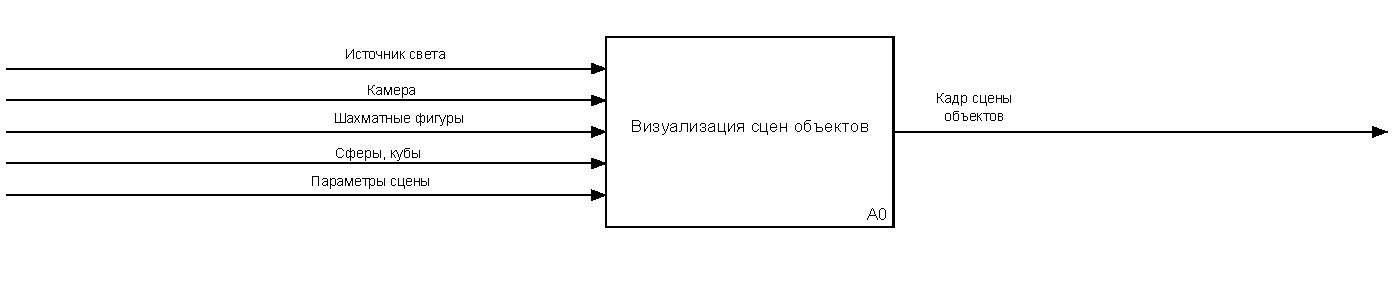
\includegraphics[width=\textwidth]{IDEF0_top}
	\caption{Верхний уровень декомпозиции задачи}
	\label{fig:IDEF0_top}
\end{figure}

\begin{figure}[H]
	\centering
	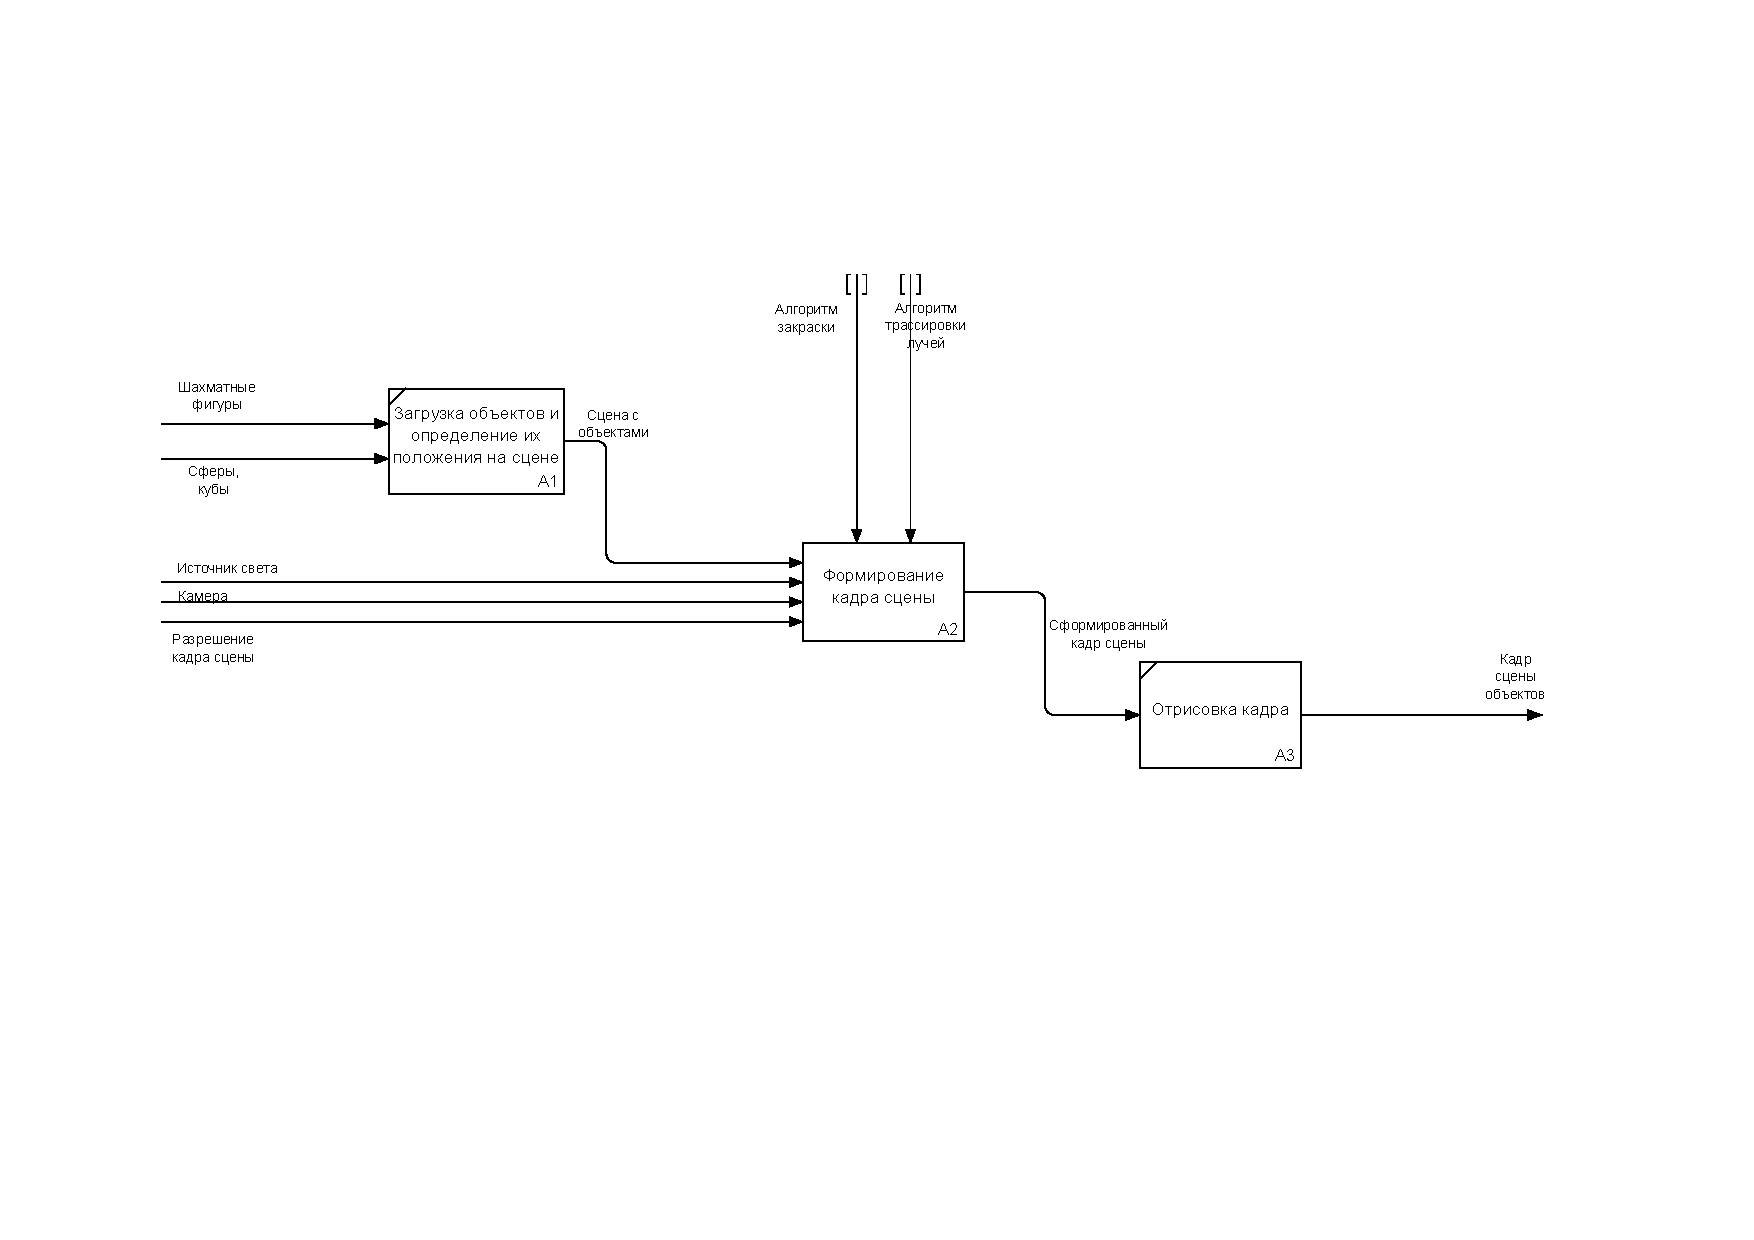
\includegraphics[width=\textwidth]{IDEF0_A0}
	\caption{Декомпозиция блока А0}
	\label{fig:IDEF0_1}
\end{figure}

\begin{figure}[H]
	\centering
	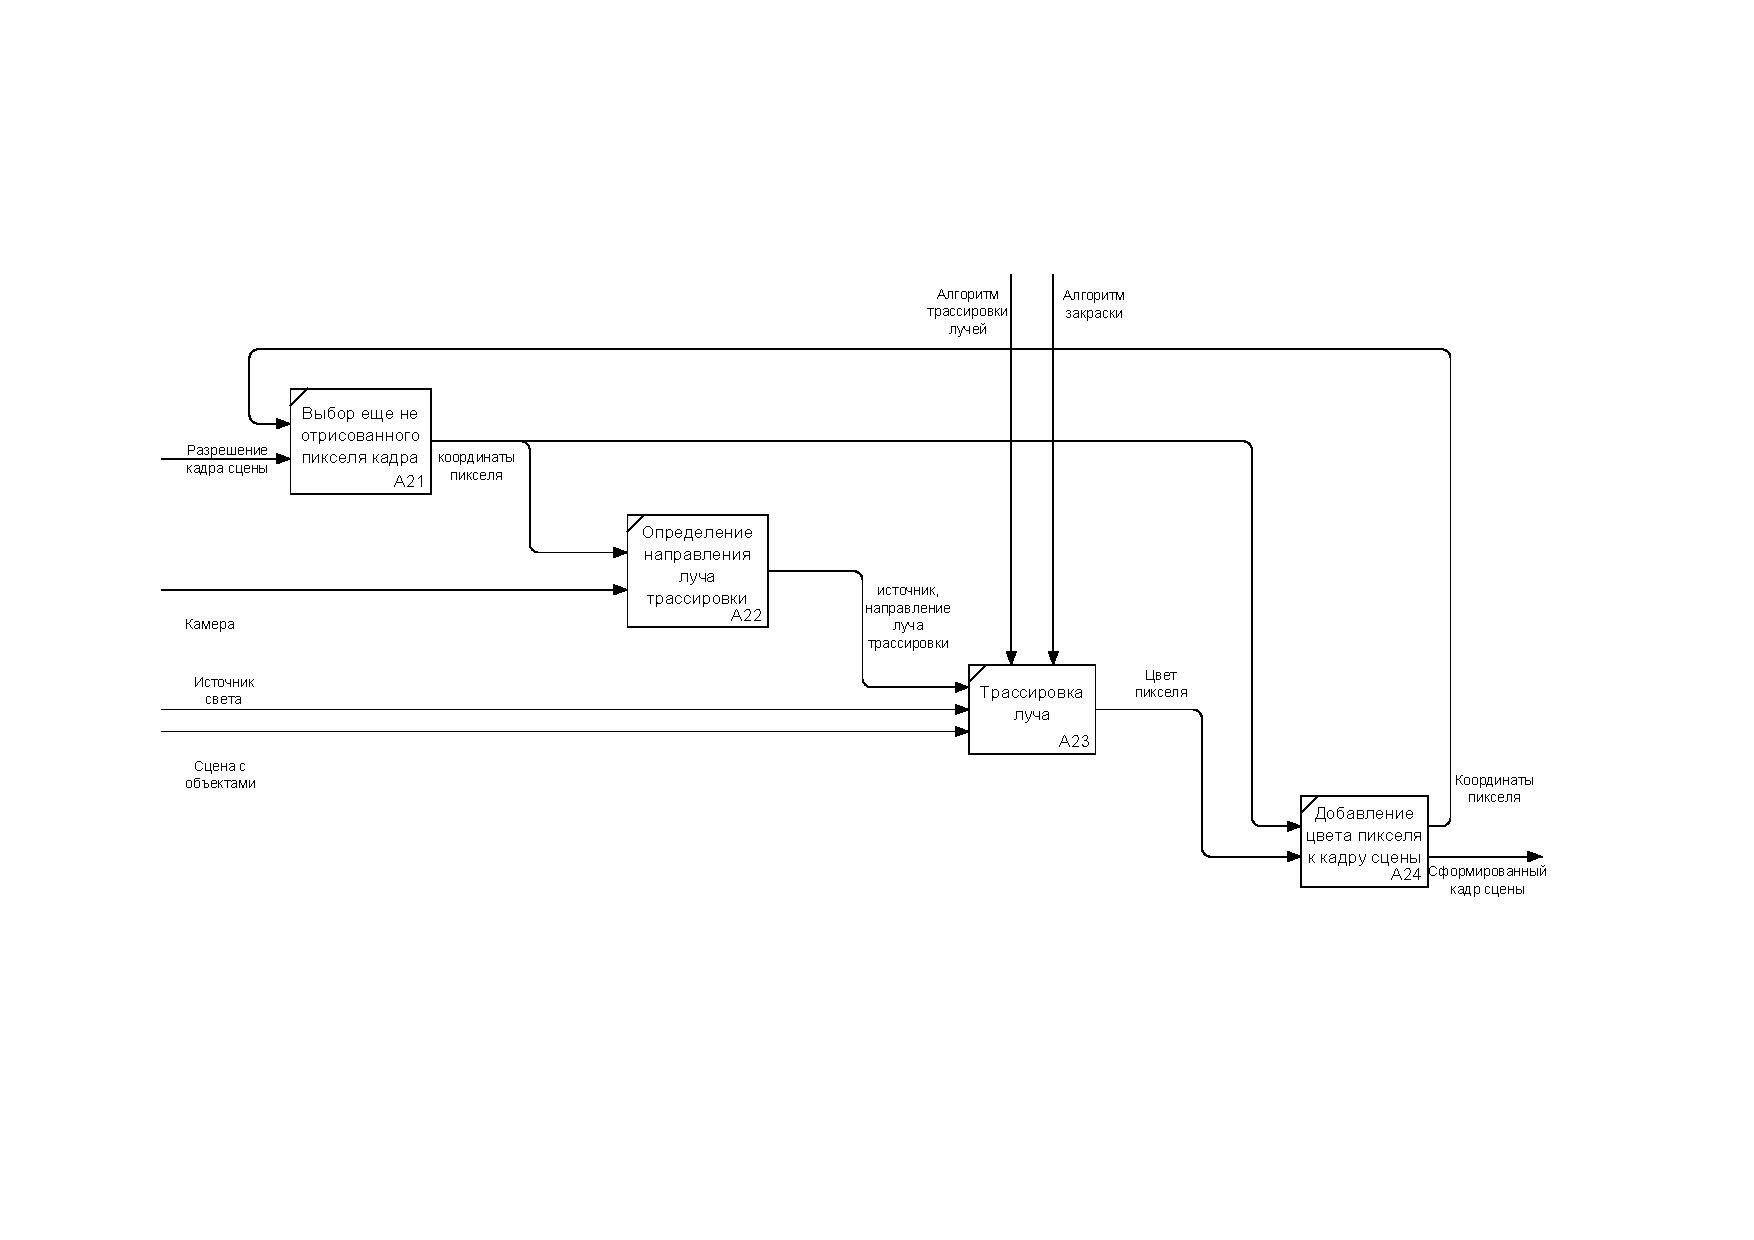
\includegraphics[width=\textwidth]{IDEF0_A2}
	\caption{Декомпозиция блока А2}
	\label{fig:IDEF0_2}
\end{figure}

Блок А23 трассировки лучей реализован в виде схемы алгоритма, приведенной на рисунке~\ref{fig:RayTracing}.


\section{Алгоритм трассировки лучей}
\begin{figure}[H]
	\centering
	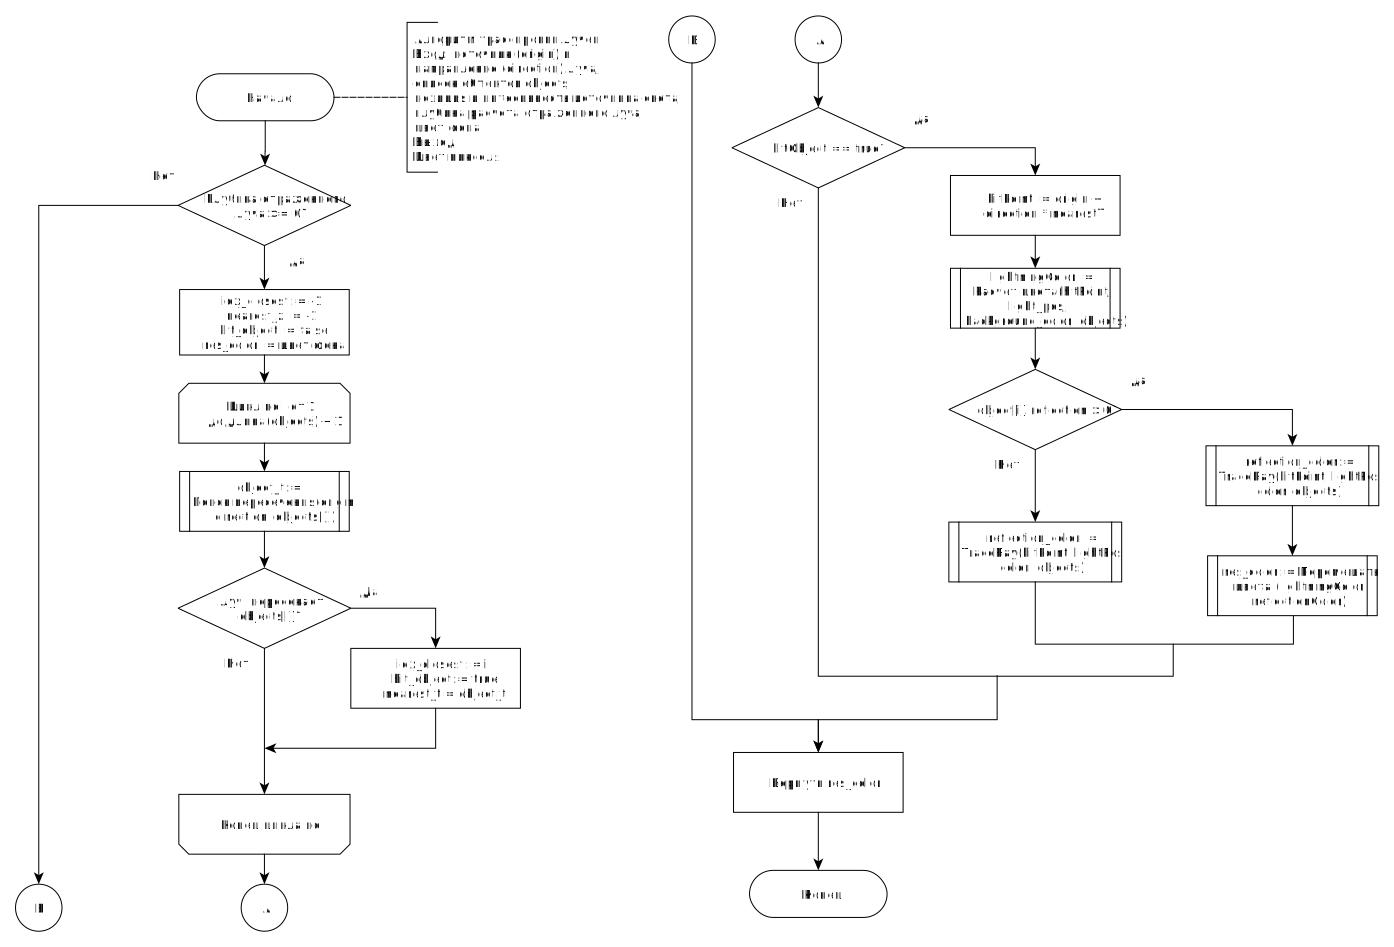
\includegraphics[height=0.9\textheight]{RayTracing}
	\caption{Схема алгоритма трассировки лучей}
	\label{fig:RayTracing}
\end{figure}

\section{Алгоритмы нахождения точки пересечения луча с объектом сцены}
Как было описано выше, в данной работе синтезируемые объекты сцены представлены одним из следующих типов:
\begin{itemize}
	\item сфера;
	\item куб;
	\item шахматные фигуры, поверхность которых состоит из треугольных полигонов.
\end{itemize}
Ниже описаны алгоритмы пересечения луча трассировки с каждым из этих типов объектов.

\subsection{Алгоритм нахождения точки пересечения луча со сферой}
Пусть $\vec{c}$ -- центр сферы, $r$ -- ее радиус. При известных $\vec{p_0}$ и $\vec{u}$ -- точке начала и вектора направления луча соответственно, можно выразить точку луча следующим образом:
\begin{equation}\label{eq:sph_1}
	\vec{p(t)} = \vec{p_0} + \vec{u} \cdot t, \qquad t \ge 0.
\end{equation}

Тогда для точки $\vec{p(t)}$ луча, лежащей на сфере, справедливо равенство
\begin{equation}\label{eq:sph_2}
	\lvert\vec{p(t)}-\vec{c}\rvert - r = 0.
\end{equation}

Подставляя \ref{eq:sph_1} в \ref{eq:sph_2} получим
\begin{equation}
	\lvert\vec{p_0} + t\cdot\vec{u} - \vec{c}\rvert - r = 0,
\end{equation} откуда получаем квадратное уравнение

\begin{equation}
	A^2\cdot t + B\cdot t + C = 0,
\end{equation}
где $A = \vec{u}$, $B = 2\vec{u}(\vec{p_0} - \vec{c})$, $C = (\vec{p_0} - \vec{c})^2 - r^2$.

Таким образом, $t$ выражается как 
\begin{equation}
	t = \frac{-B \pm \sqrt{B^2-4C}}{2}, 
\end{equation}
при этом выбирается меньшее $t$ (ближайшая точка) и проверяется на положительность.

На рисунке \ref{fig:RaySphere} приведена схема алгоритма, реализующая описанные вычисления.

\begin{figure}[H]
	\centering
	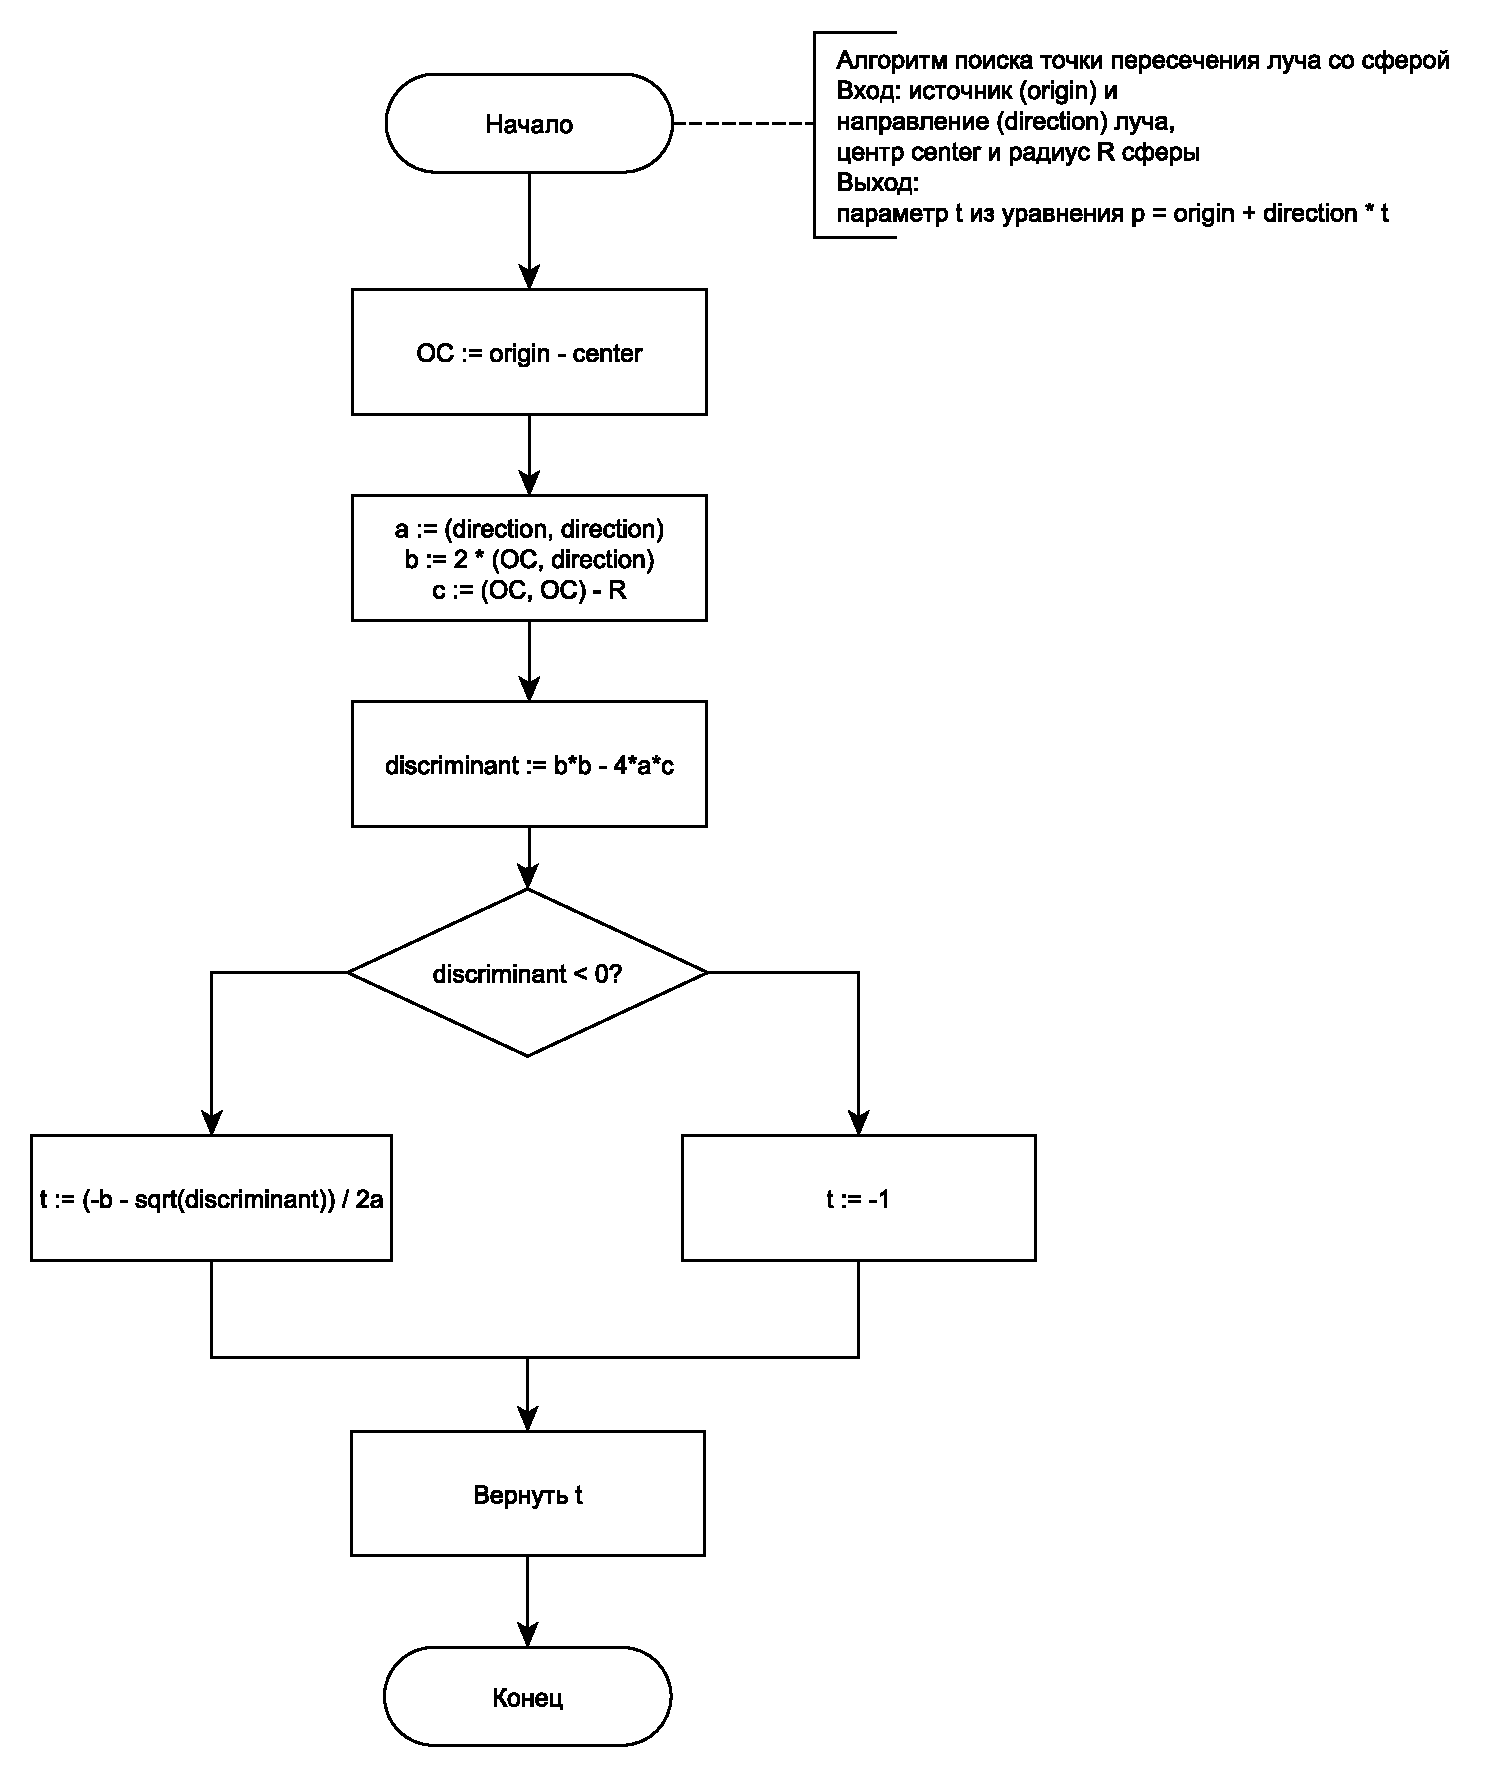
\includegraphics[height=0.5\textheight]{SphereIntersection}
	\caption{Схема алгоритма нахождения точки пересечения луча и сферы}
	\label{fig:RaySphere}
\end{figure}

\subsection{Алгоритм нахождения точки пересечения луча и куба}
Алгоритм нахождения точки пересечения луча с кубом использует представление луча в форме, описанной формулой \ref{eq:sph_1}, а также идею последовательного обрезания луча каждой из граней куба~\cite{lit7}.
Алгоритм представлен на схемах~\ref{fig:CubeIntersection_1}-\ref{fig:CubeIntersection_2}.
\begin{figure}[H]
	\centering
	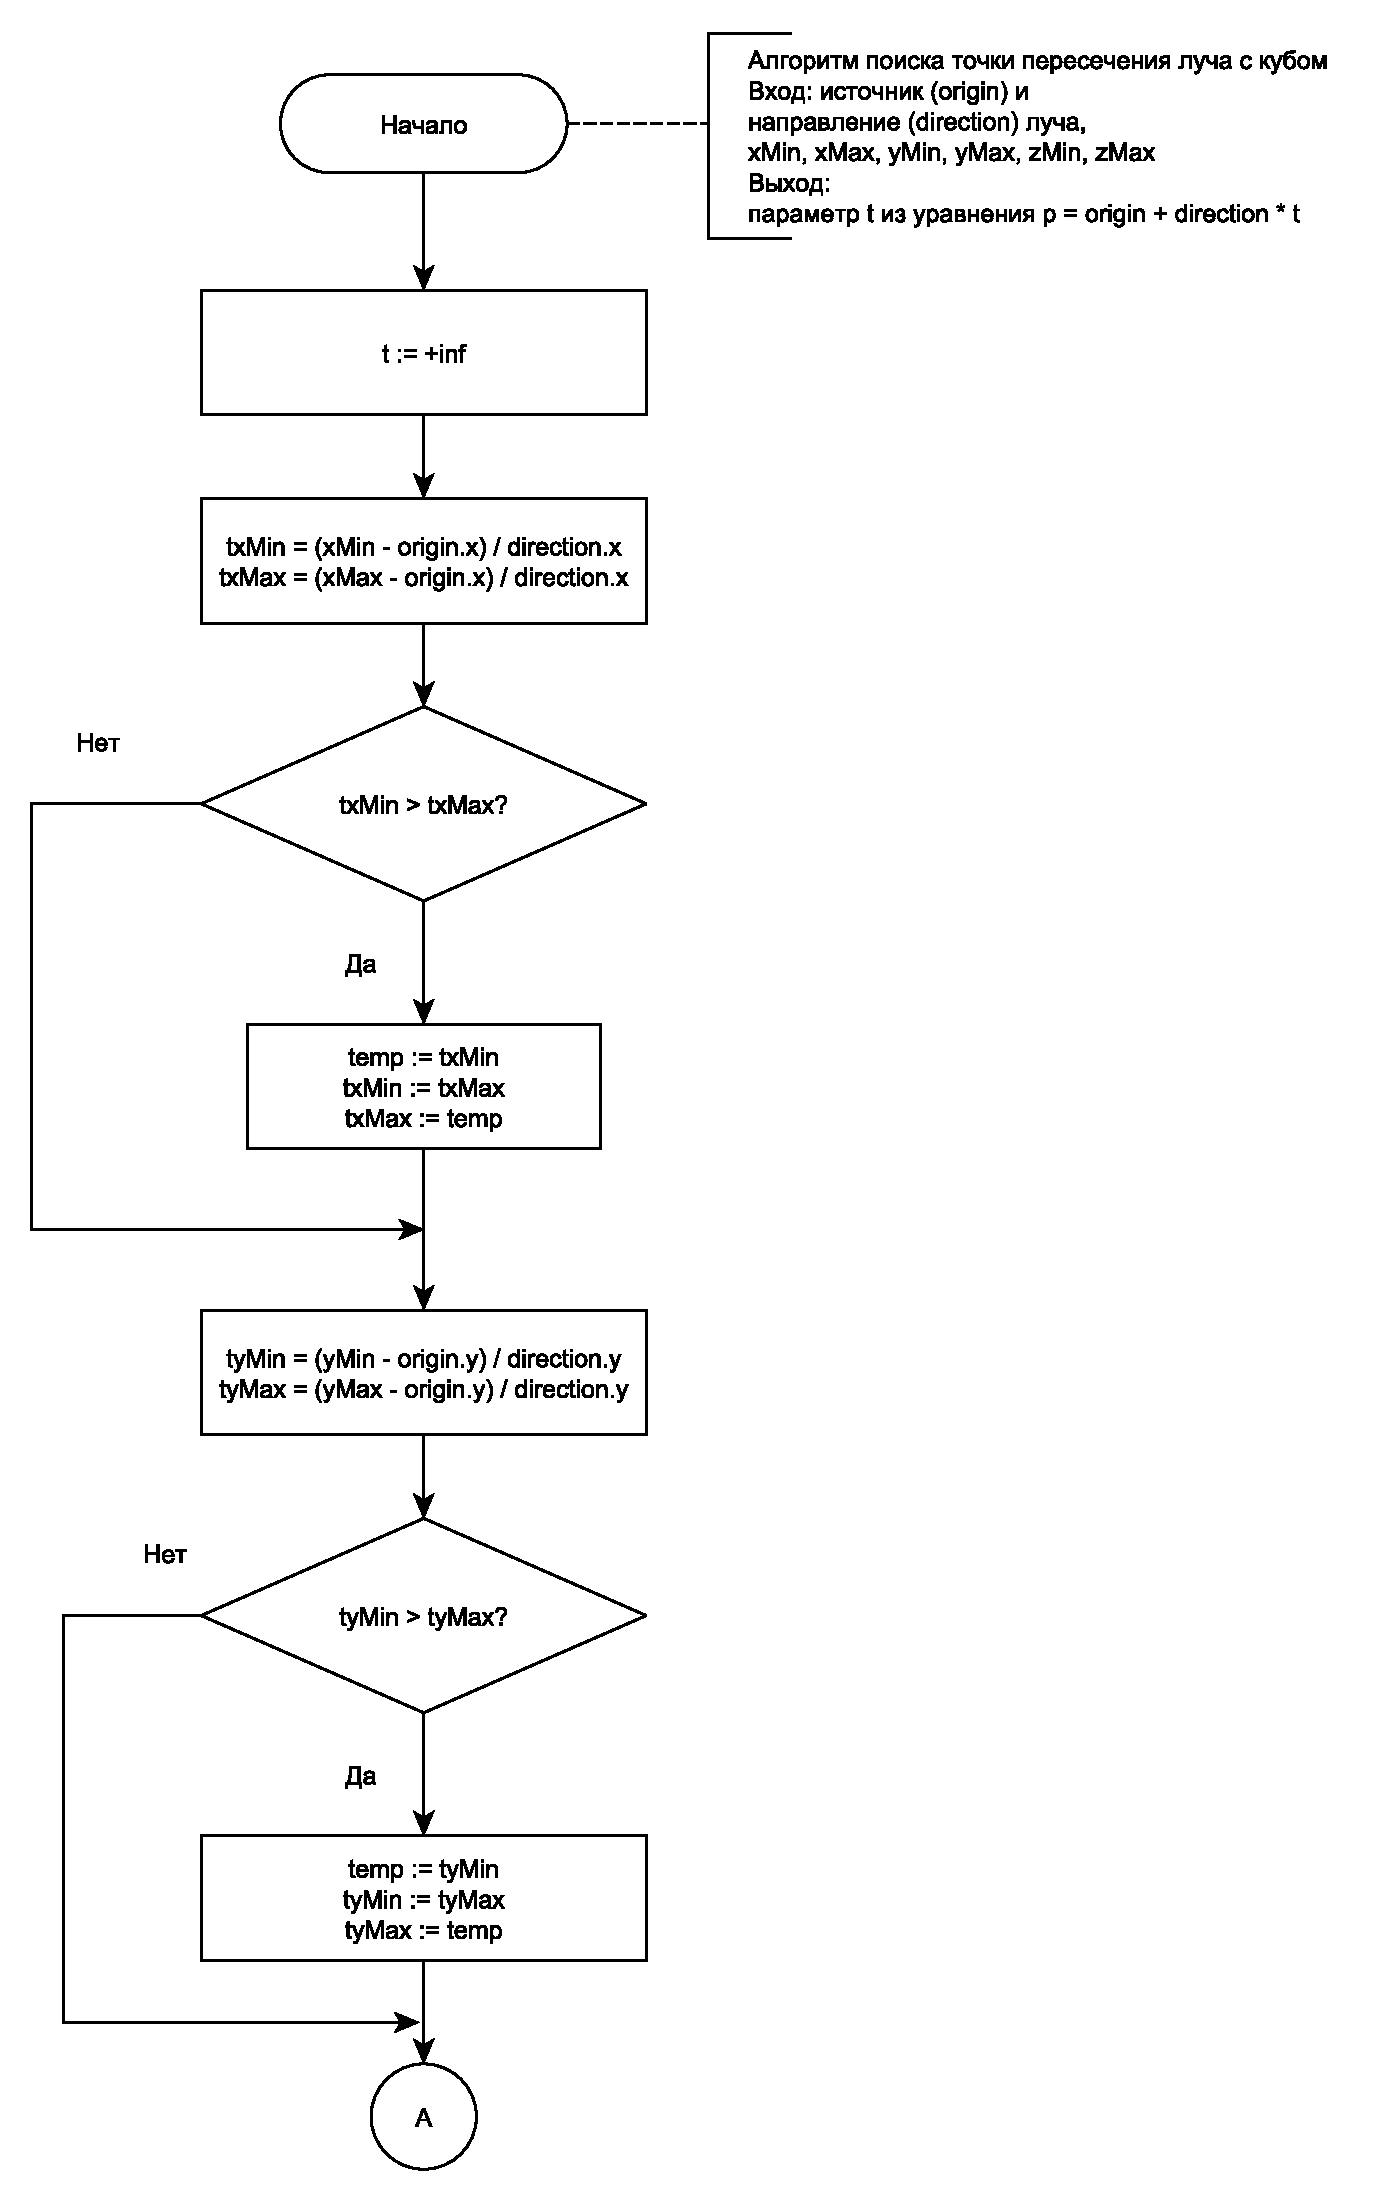
\includegraphics[height=0.7\textheight]{CubeIntersection_1}
	\caption{Схема алгоритма нахождения точки пересечения луча и сферы}
	\label{fig:CubeIntersection_1}
\end{figure}

\begin{figure}[H]
	\centering
	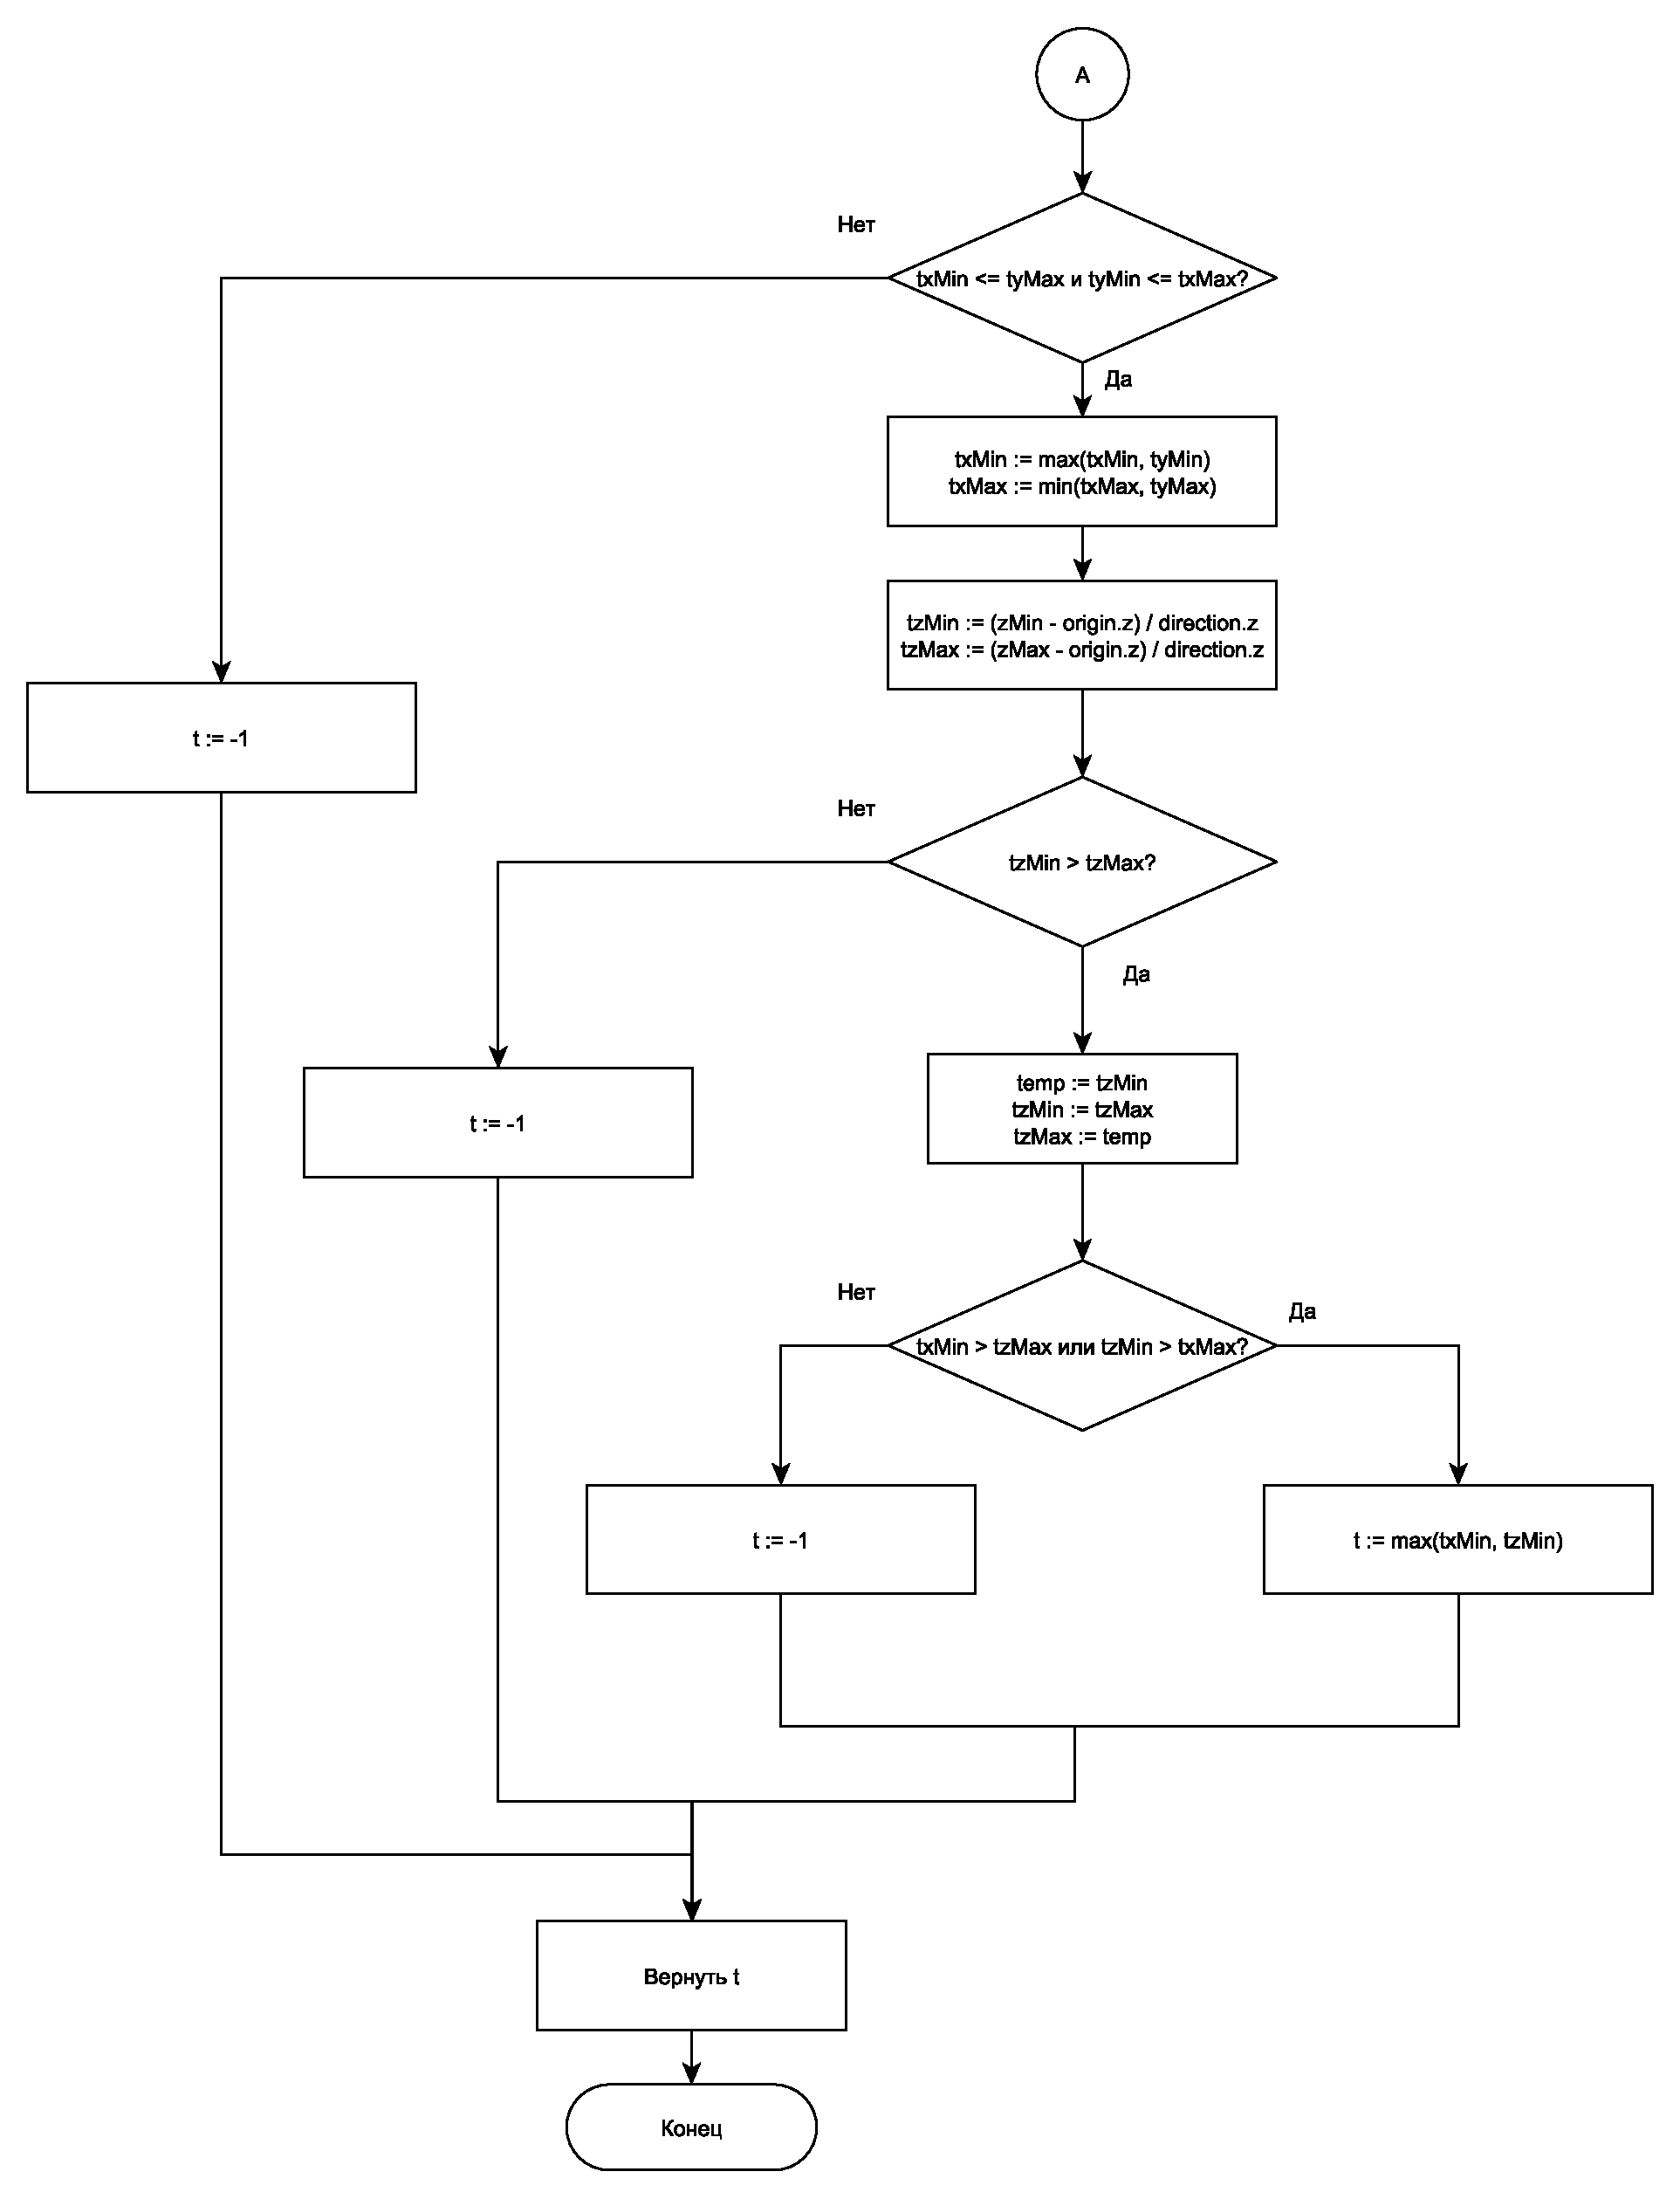
\includegraphics[width=0.9\textwidth]{CubeIntersection_2}
	\caption{Схема алгоритма нахождения точки пересечения луча и сферы}
	\label{fig:CubeIntersection_2}
\end{figure}

\subsection{Алгоритм нахождения точки пересечения луча и шахматной фигуры}
Поскольку модели шахматных фигур состоят из треугольных полигонов, задача нахождения точки пересечения луча и фигуры включает в себя подзадачу поиска точки пересечения с треугольником. Для решения задачи был выбран алгоритм Моллера~---~Трумбора, позволяющий решить задачу без предварительного вычисления уравнения плоскости, содержащей треугольник~\cite{lit8}.

\begin{figure}[H]
	\centering
	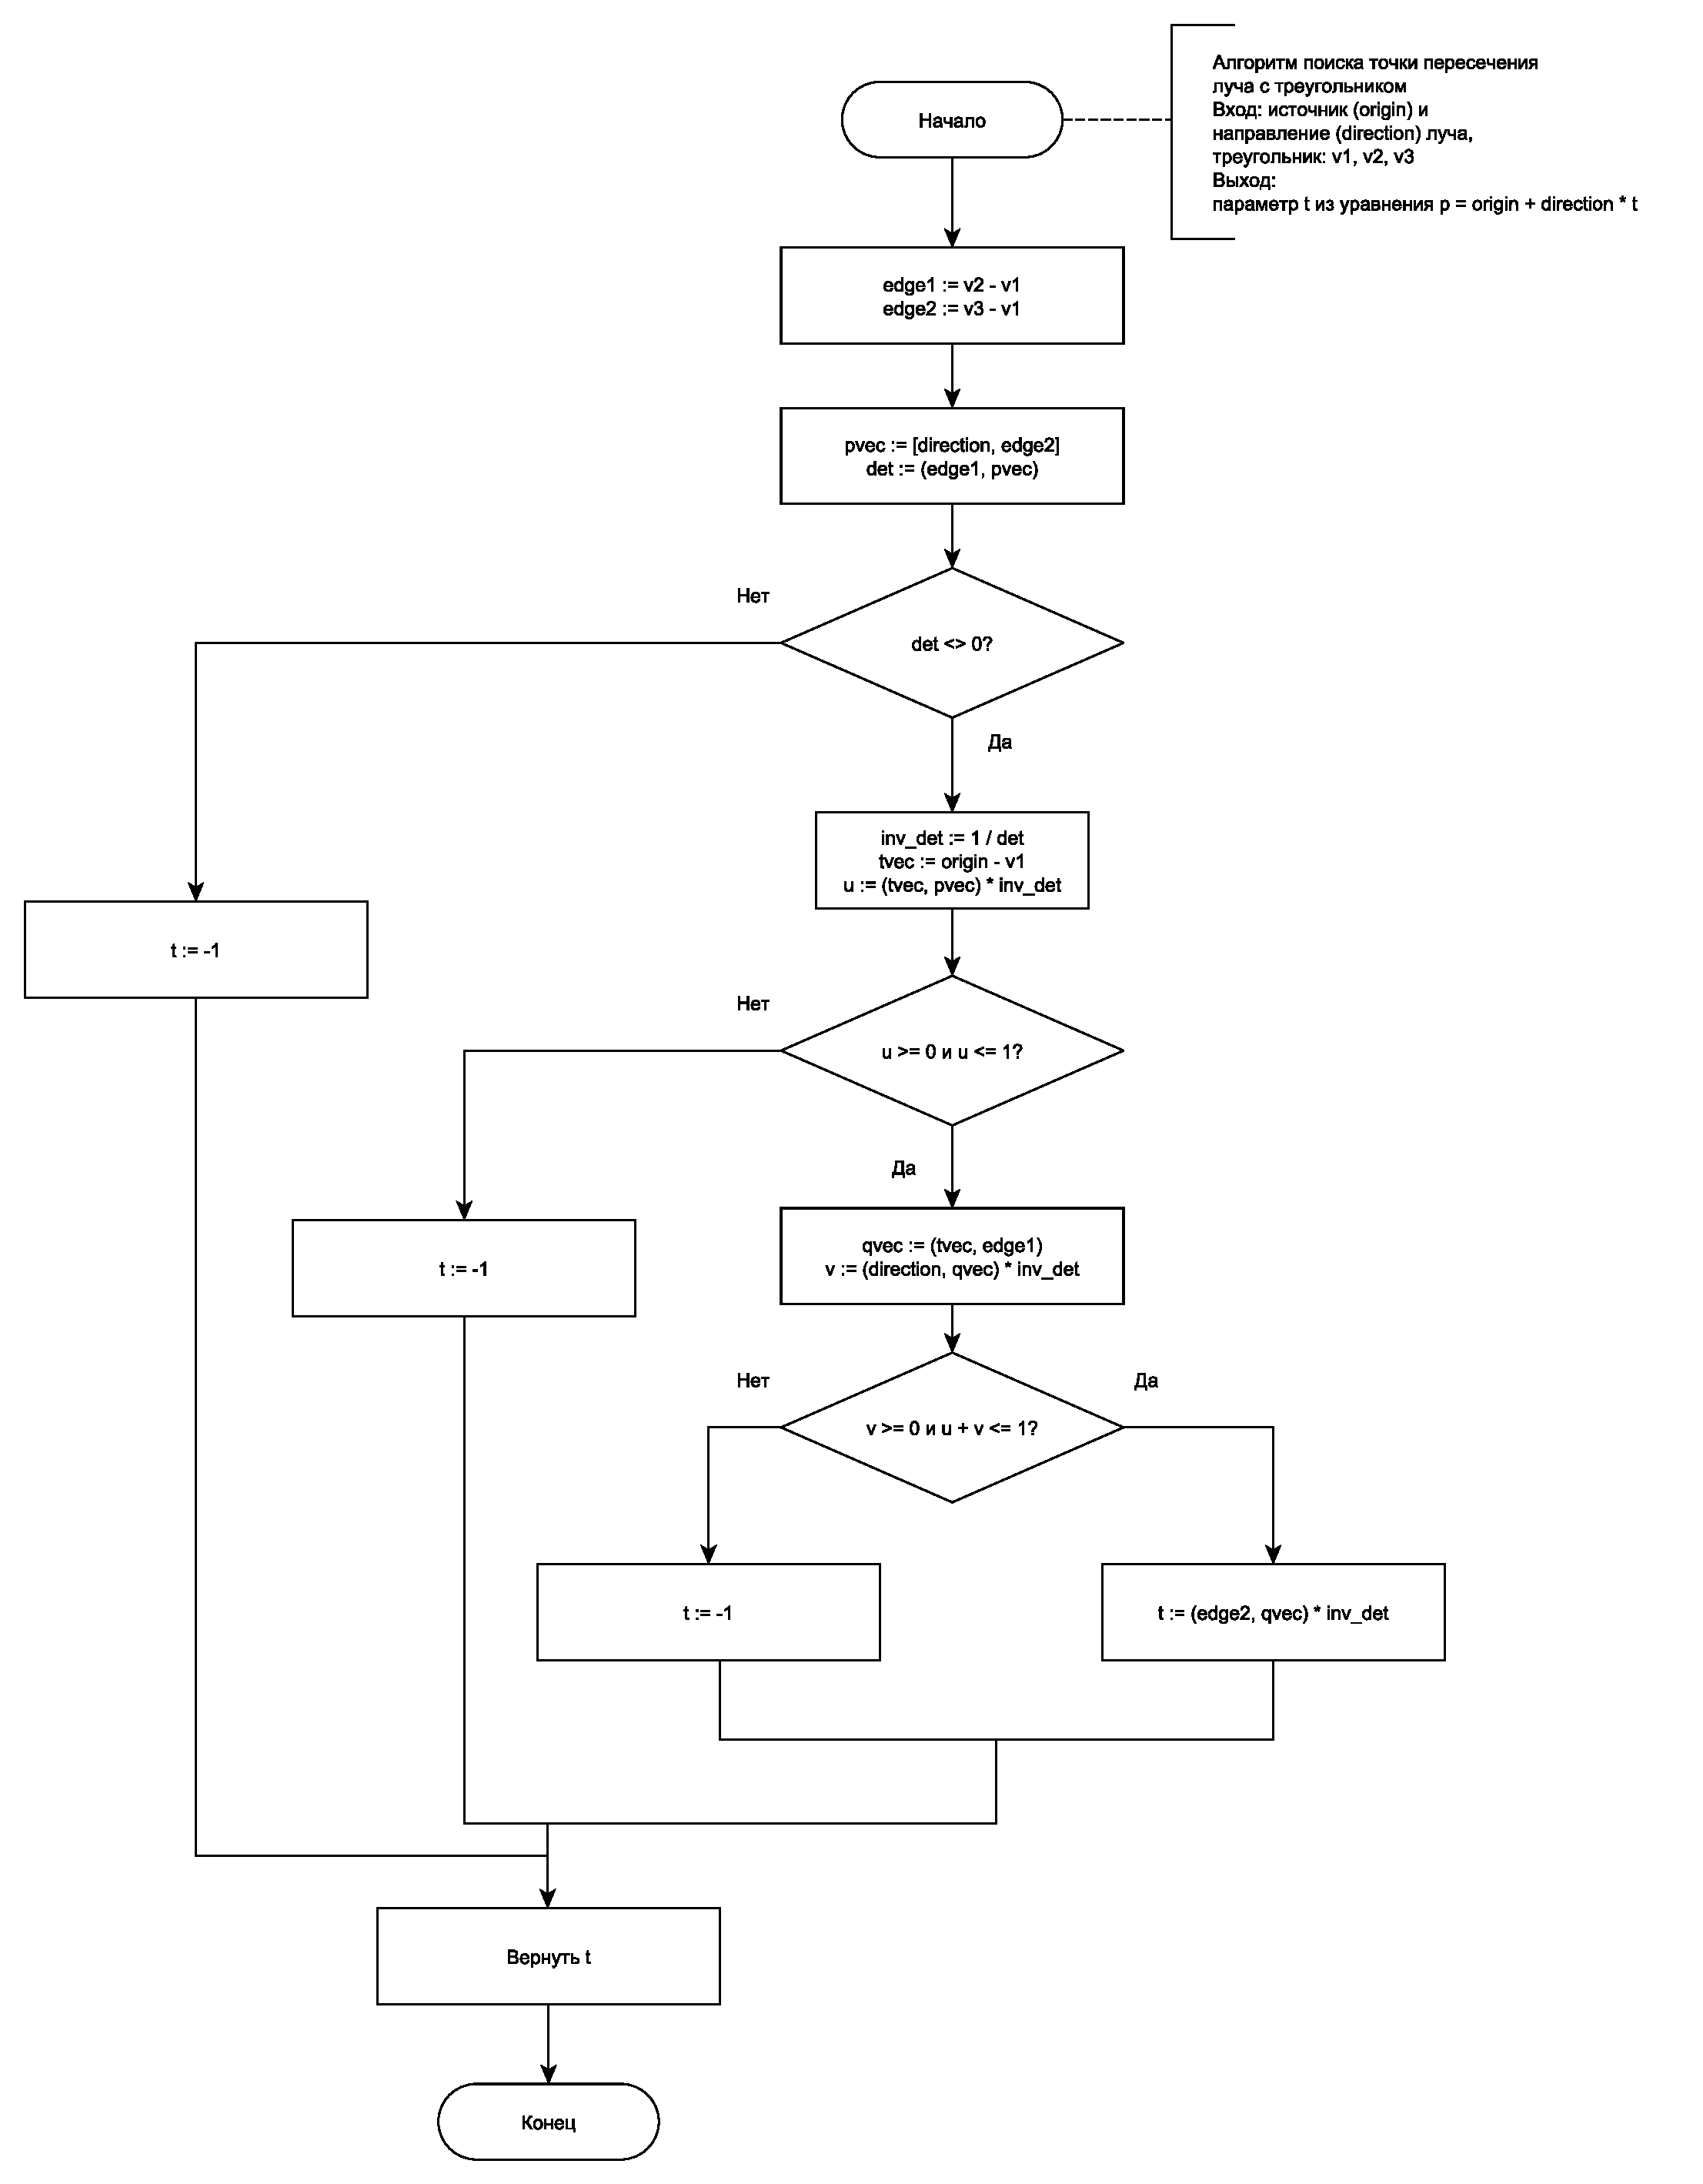
\includegraphics[width=0.9\textwidth]{TriangleIntersection}
	\caption{Схема алгоритма нахождения точки пересечения луча и треугольника}
	\label{fig:TriangleIntersection}
\end{figure}

Алгоритм нахождения точки пересечения луча и шахматной фигуры использует предварительный расчет описанной сферы при создании шахматной фигуры, и далее использует сферу, проверяя пересечение луча с описанной сферой прежде чем итерироваться по всем треугольникам фигуры: если луч не пересекает описанную сферу, то он не может пересечь фигуру. При описанной проверке используется алгоритм нахождения точки пересечения луча со сферой~\ref{fig:RaySphere}.

\begin{figure}[H]
	\centering
	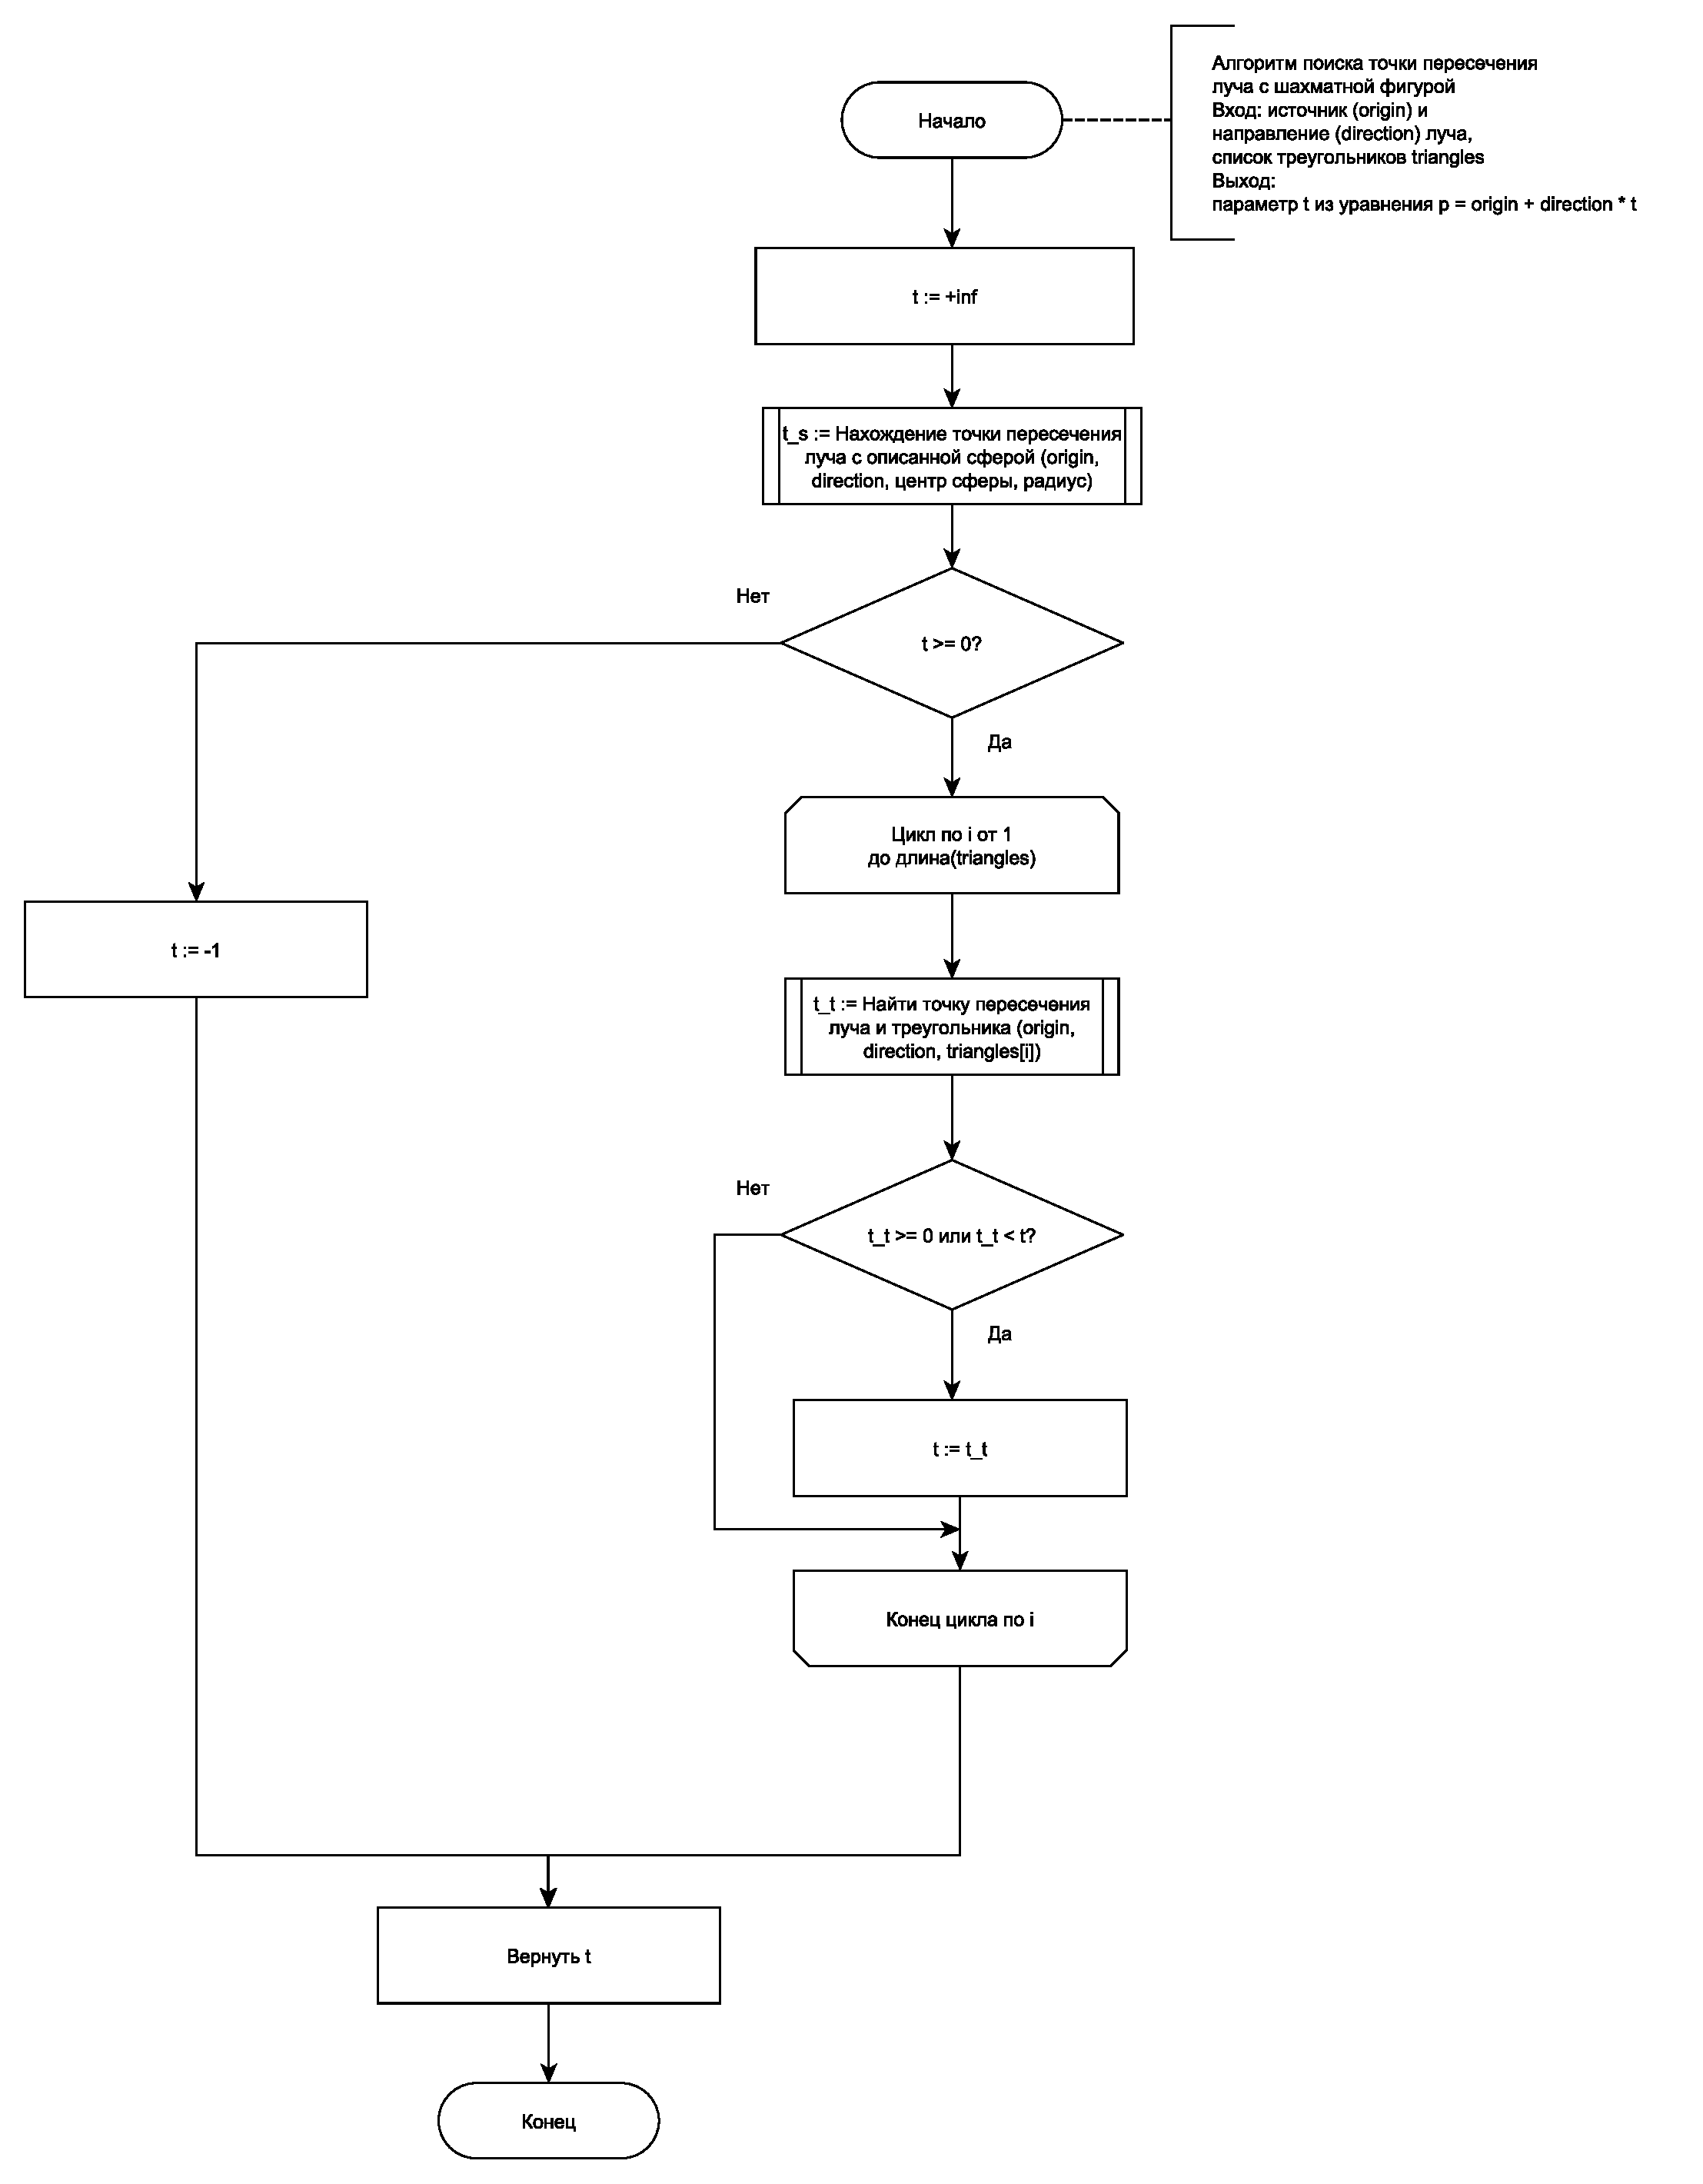
\includegraphics[width=0.9\textwidth]{ChessIntersection}
	\caption{Схема алгоритма нахождения точки пересечения луча и шахматной фигуры}
	\label{fig:ChessIntersection}
\end{figure}

\section*{Вывод}
В данном разделе были формализованы требования к реализуемому ПО, объекты сцены и их структура, приведена декомпозиция задачи, а также рассмотрены схемы алгоритмов визуализации сцены объектов методом трассировки лучей.

\clearpage
